\section{phi of t}
\subsection{Effective source}
\subsection{World tube}
\begin{figure}
\includegraphics{worldTubeItself}
\caption{Spatial slice of the world tube window function.}
\end{figure}
\begin{figure}
  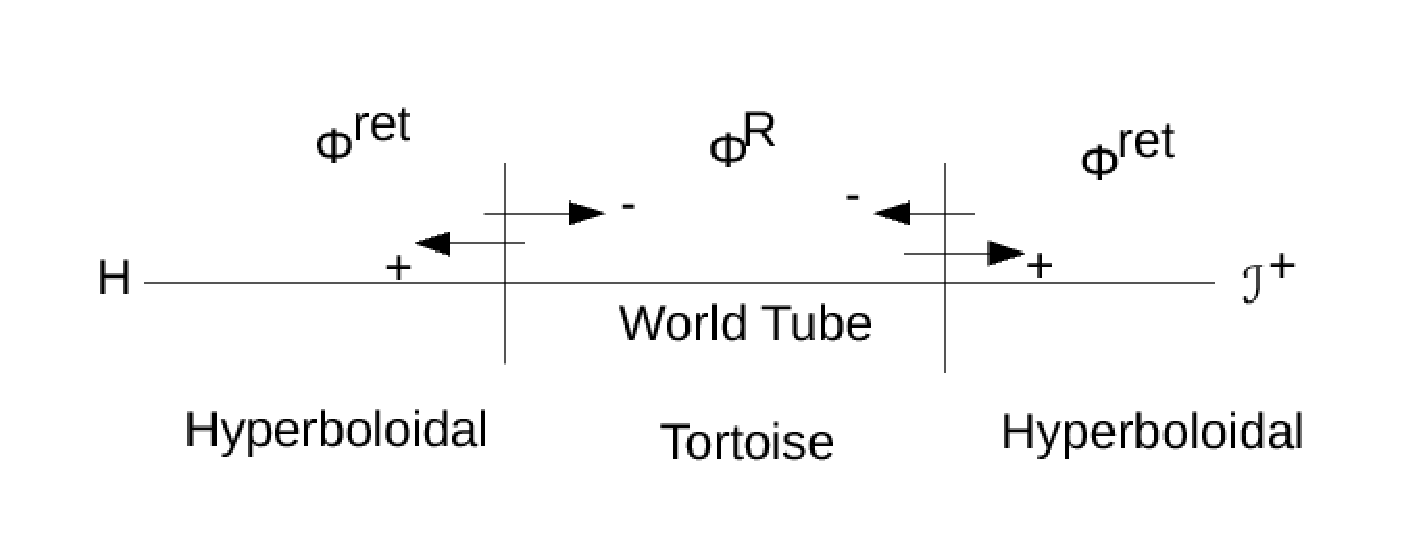
\includegraphics{WorldTube}
  \caption{Add or subtract the singular field to either side of the world tube boundary before performing the time dependent coordinate transform (or inverting it) to obtain the retarded field in the exterior region and the regularized field in the interior region.}

\end{figure}


\subsection{Comparison between C++ and Fortran codes}
\begin{figure}
  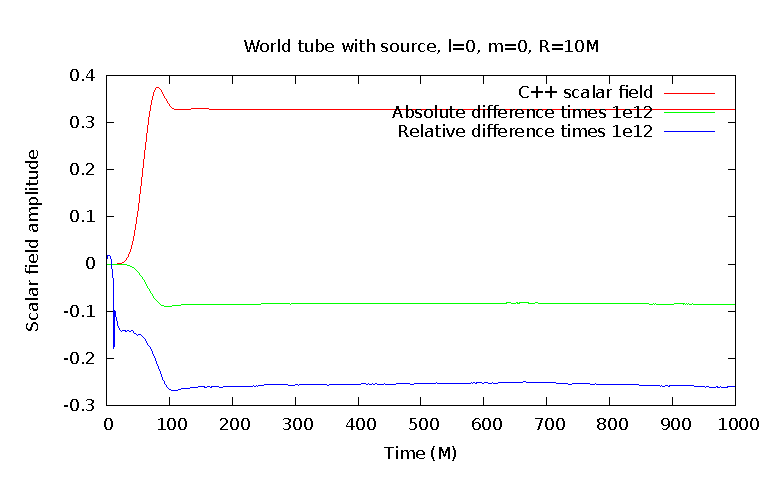
\includegraphics{wtcircl0m0}
  \caption{Comparison between Fortran and C++ codes for a particle on a circular orbit, l=0, m=0.}
\end{figure}
\begin{figure}
  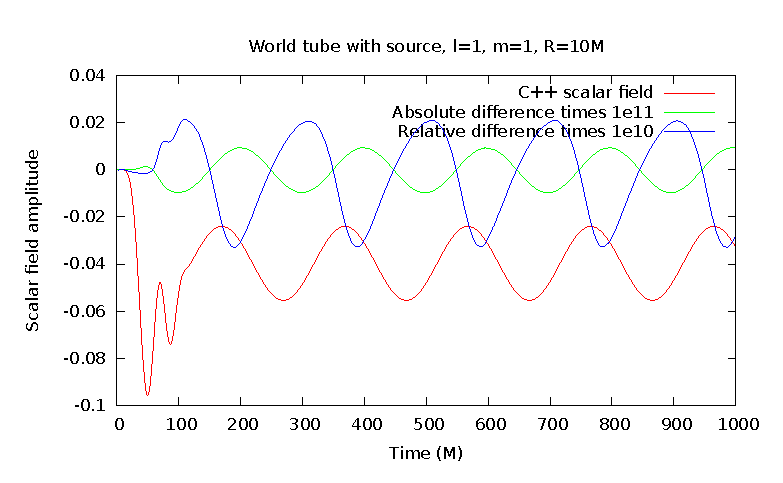
\includegraphics{wtcircl1m1}
  \caption{Comparison between Fortran and C++ codes for a particle on a circular orbit, l=1, m=1.}
\end{figure}
\begin{figure}
  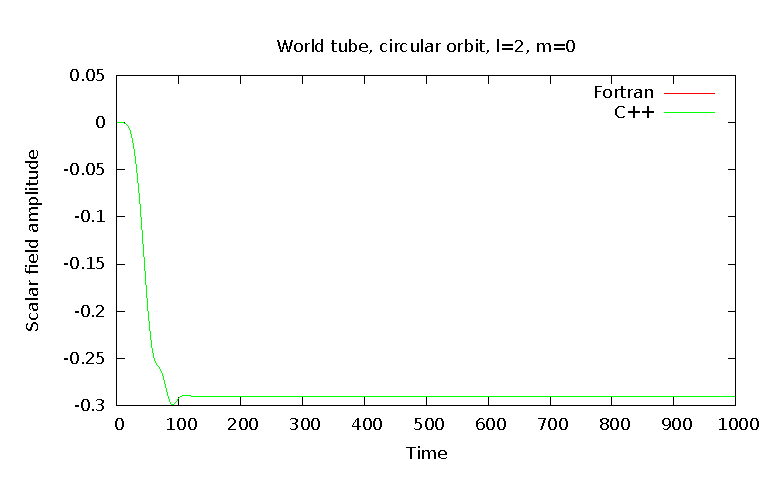
\includegraphics{wtcircl2m0}
  \caption{Comparison between Fortran and C++ codes for a particle on a circular orbit, l=2, m=0.}
\end{figure}
\begin{figure}
  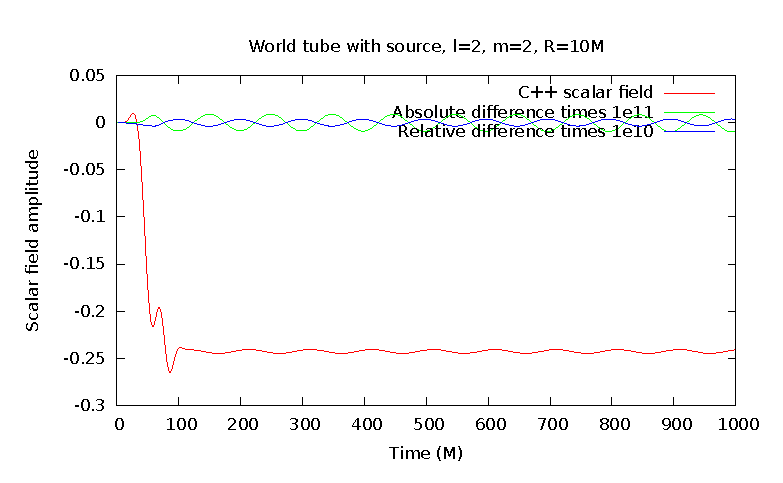
\includegraphics{wtcircl2m2}
  \caption{Comparison between Fortran and C++ codes for a particle on a circular orbit, l=2, m=2.}
\end{figure}
